
%(BEGIN_QUESTION)
% Copyright 2012, Tony R. Kuphaldt, released under the Creative Commons Attribution License (v 1.0)
% This means you may do almost anything with this work of mine, so long as you give me proper credit

Identify the two transmitters used in the cascade liquid level control for the ``rundown tank'' in this ammonium nitrate production process, and also identify what would happen to the rundown tank level if the instrument air supply to the ammonium nitrate flow control valve failed (i.e. the supply air pressure fell to 0 PSI).  Assume the flow transmitter for that loop is direct-acting and that the flow controller for that loop is reverse acting:

$$\epsfysize=7.5in \includegraphics[width=15.5cm]{i01142x01.eps}$$

\underbar{file i01142}
%(END_QUESTION)





%(BEGIN_ANSWER)

{\it 3 points for each correct transmitter identification, 4 points for correct consequence of air failure.}

\vskip 10pt

Rundown tank level transmitter = {\bf LT-26}

\vskip 10pt

Ammonium nitrate flow transmitter = {\bf FT-25}

\vskip 10pt

If instrument air fails, the rundown tank level {\bf increase} because FV-25 is fail-closed (FC) and there will be no way to get ammonium nitrate out of the rundown tank.

%(END_ANSWER)





%(BEGIN_NOTES)


{\bf This question is intended for exams only and not worksheets!}.

%(END_NOTES)

